В настоящем разделе описывается лабораторная установка, на экспериментальных данных которой будет верифицироваться численная модель. Данная установка была разработана в ИДГ РАН~\cite{trimonova2017, trimonova2018}. К ее основным возможностям можно отнести: исследования гидроразрыва пласта и сопуствующих ему процессов, создание трехмерного напряженно-деформированного состояния, изучение нестабильных трещин на нагнетательных скважинах, моделирование взаимодействия трещин и многое другое. Ниже будут описаны особенности уставновки, важные с точки зрения математического моделирования протекающих в ней процессов.

\subsection{Описание установки}
Конструктивно установка для моделирования процессов в плоском коллекторе состоит из верхней и нижней крышек, в кольцевом углублении которых фиксируется боковина.      Схематический внешний вид установки показан на рисунке~\ref{device:pict}. Между собой крышки скрепляются шестнадцатью шпильками, которые на рисунке не показаны. Толщина крышек составляет  75~мм при наружном диаметре 600~мм. Высота боковины равна 70~мм при внутреннем диметре 430~мм и толщине стенки 25~мм.

\begin{figure}[hb]
\begin{center}
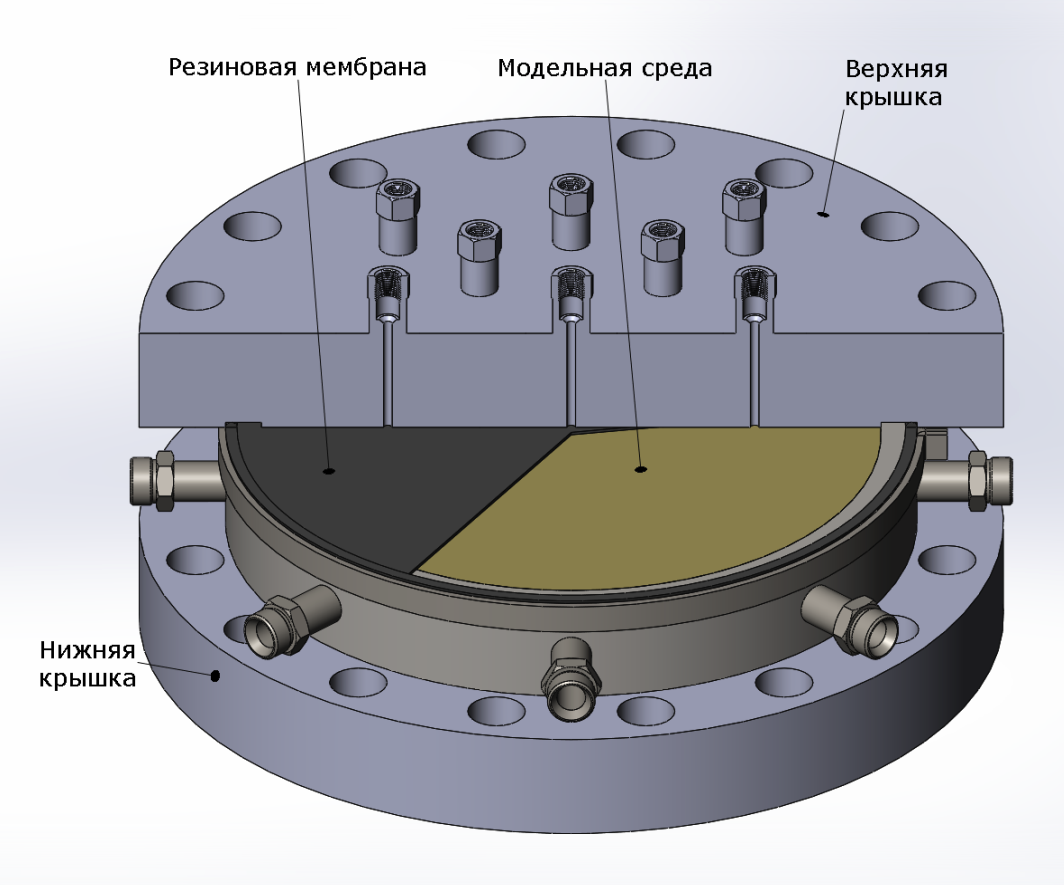
\epsfig{file=figs/picts/1, width=.5\textwidth}
\end{center}
\caption{Схема плоской модельной установки}\label{device:pict}
\end{figure}

Основные детали установки изготовлены из нержавеющей стали. Крышки размещаются на станине, что позволяет свободно их переворачивать и перемещать верхнюю крышку в свой ложемент. Это дает возможность проводить необходимые операции, связанные с подготовкой и проведением экспериментов, несмотря на значительную массу составных частей установки (масса крышек превышает 160 кг). Фотографии общего вида установки представлены на рисунках~\ref{device1:pict}.

\begin{figure}[hb]
\begin{center}
\begin{tabular}{cc}
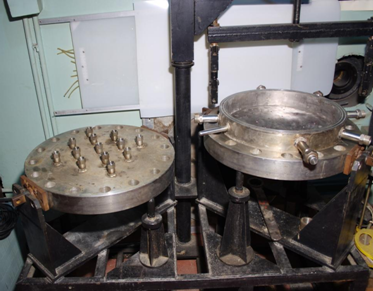
\epsfig{file=figs/picts/2, height=6cm} &
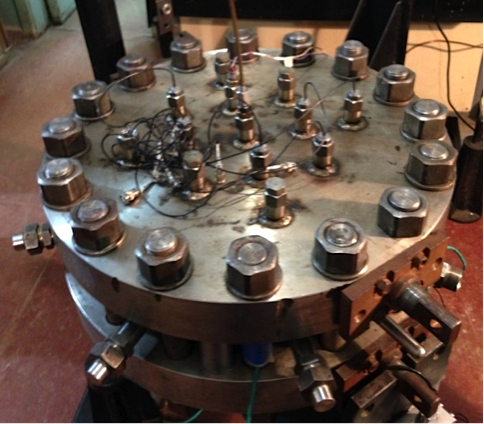
\epsfig{file=figs/picts/3, height=6cm} 
\end{tabular}
\end{center}
\caption{Общий вид экспериментальной установки}\label{device1:pict}
\end{figure}

Перед началом эксперимента в установку заливается гипс. Затвердевая, он образует модельную среду. Верхняя крышка отделена от образца резиновой мембраной. По периметру мембраны расположены резиновое кольцо и опорный хомут, которые создают герметичное пространство между мембраной и крышкой (рис. ~\ref{device:pict}). Это пространство заполняется водой под давлением, что позволяет моделировать литостатическое давление в модели коллектора. Давление над мембраной поддерживается при помощи разделительного цилиндра, верхняя часть которого заполнена сжатым азотом под необходимым давлением, а нижняя водой. 

Горизонтальное нагружение модели обеспечивается с помощью герметичных камер, расположенных на поверхности боковой стенки. Фотография установки (вид сверху) с боковыми камерами представлен на рисунке ~\ref{device2:pict}. Камеры изготовлены из листовой меди толщиной 0,3~мм. Внутренняя полость камер имеет толщину 3~мм, высота камеры на 2~мм меньше высоты боковой стенки. Длина дуги камеры составляет примерно $80^\circ$. Патрубок камеры через герметичное уплотнение выводится из боковой стенки наружу. Камеры зафиксированы на боковой поверхности кольца с помощью силиконового герметика. Боковое нагружение осуществляется за счет закачки газа или жидкости в попарно противоположные камеры.

\begin{figure}[hb]
\begin{center}
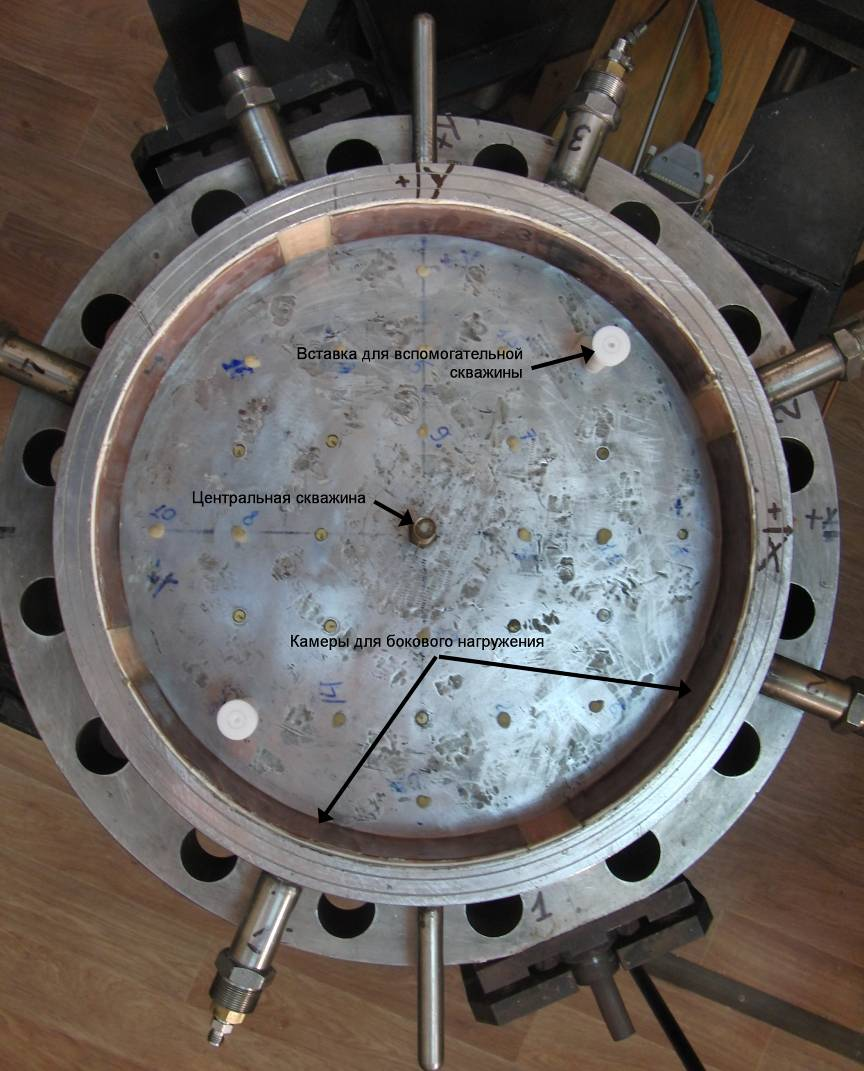
\epsfig{file=figs/picts/4, width=.4\textwidth}
\end{center}
\caption{Фотография установки: вид сверху}\label{device2:pict}
\end{figure}

В обеих крышках и в боковине просверлены сквозные технологические отверстия диаметром 6~мм, оснащенные с внешней стороны приваренными резьбовыми штуцерами. В верхней крышке находится 29 отверстий, в нижней – 13, в боковине – 6. Эти отверстия могут использоваться как для монтажа различных датчиков, так и для обеспечения отбора или закачки флюида в коллектор. Поровое давление в модели измеряется через технологические отверстия, расположенные в нижней крышке установки, с помощью тензопреобразователей. Технологические отверстия заполняются водой и перед заливкой гипса закрываются поролоновыми вкладышами. Вкладыши на 4…5 мм выступают над поверхностью нижнего основания и после заливки гипса оказываются вмонтированы в него, обеспечивая передачу порового давления к тензопреобразователям. Схема расположения датчиков показана на рисунке ~\ref{device3:pict}.

\begin{figure}[hb]
\begin{center}
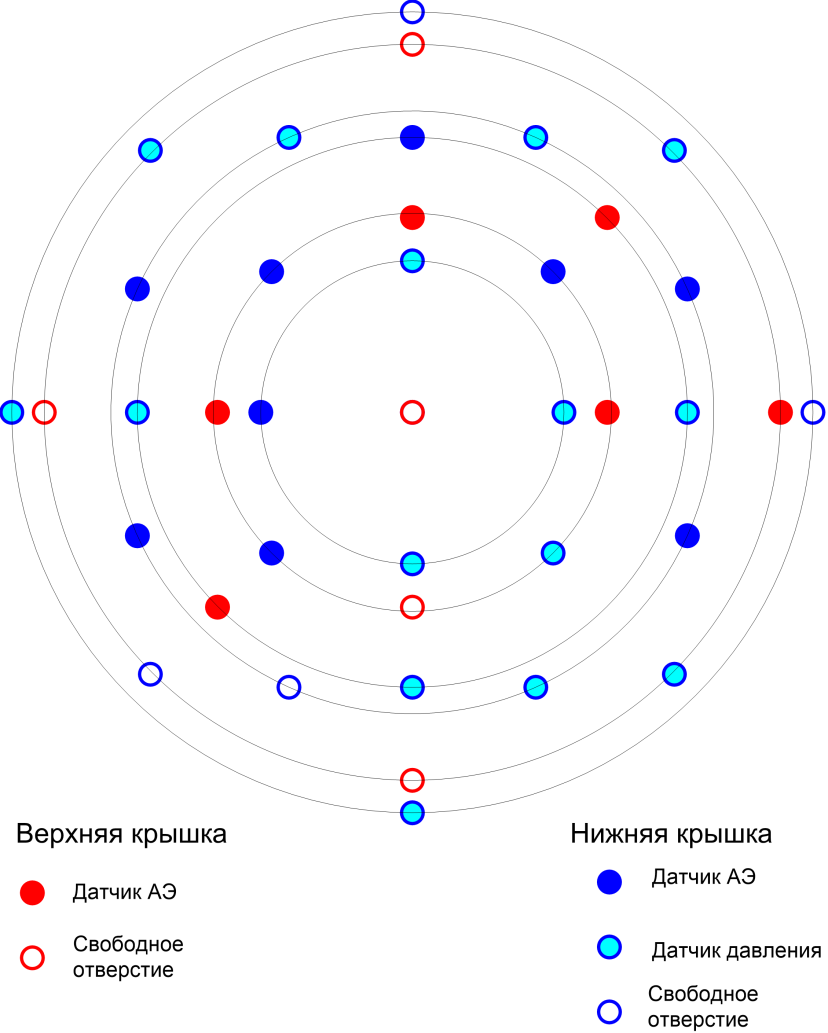
\epsfig{file=figs/picts/5, width=.5\textwidth}
\end{center}
\caption{Схема расположения датчиков в нижней и верхней крышках}\label{device3:pict}
\end{figure}

Вспомогательные скважины, необходимые для прокачки насыщенного раствора сульфата кальция (гипса) через образец и для создания поля порового давления в нем, формируются при отливке образца путем помещения в него заранее вставок из фторопласта диаметром 15~мм в центрально симметричные технологические отверстия (рисунок \ref{device2:pict}). После затвердевания гипса вставки вынимаются, а сами образовавшиеся скважины закрываются фторопластовыми крышками.

Центральная скважина представляет собой латунную трубку диаметром 16~мм, которая герметично вставляется в нижнюю крышку установки. Трубка имеет возможность свободно вращаться вокруг вертикальной оси, позволяя ориентировать затравку трещины ГРП в заданном направлении. Верхний торец трубки закрыт винтовой пробкой. В средней части трубки проделана вертикальная прорезь, в которую вставляется сложенная вдвое тонкая латунная сетка, служащая затравкой трещины ГРП. Размер лепестков сетки составляет 8х8~мм. Углы лепестков срезаны примерно на 2~мм. После заливки гипса мы получаем обсаженную скважину с перфорированной стенкой и затравкой трещины ГРП.

Эксперименты, как правило, проводятся на третьи сутки после заливки гипса, пока не высохнет гипс. После сборки экспериментальной установки модель нагружается небольшим вертикальным давлением (1…1,5 МПа), затем задается необходимое давление в боковых камерах. После этого вертикальное давление поднимается до рабочего значения. Перед началом эксперимента проводится дополнительное насыщение гипсового образца жидкостью под постоянным давлением закачки около 1~МПа на технологической нагнетательной скважине. Критерием завершения процесса насыщения служит стабилизация расхода на добывающей скважине и давлений в точках измерения порового давления. Обычно насыщение продолжается около 1 часа. Непосредственно после завершения процесса насыщения проводится эксперимент по ГРП.

\subsection{Используемый материал}

Выбор среды, моделирующей коллектор, определяется постановкой решаемых экспериментальных задач. Целью данного исследования является экспериментальное моделирование ГРП с возможностью переноса результатов экспериментов на пластовые условия. Но помимо критериев подобия, отвечающих за возможность такого переноса~\cite{cleary1994}, важнейшую роль играют технологические факторы, связанные с возможностью изготовления экспериментальных образцов. С этой точки зрения смесь на основе гипса с добавкой портландцемента является хорошим выбором. Хорошая текучесть смеси и отсутствие усадки при затвердевании позволяет добиться плотного контакта со стенками установки. Для замедления схватывания гипса в воду для приготовления смеси добавляется лимонная кислота в концентрации 2 г/дм$^3$. Описание экспериментов по определению прочностных и фильтрационных характеристик образца можно найти  в~\cite{trimonova2017, trimonova2018}. 

Следующие величины были получены экспериментально:
\begin{description}
%
\item $\nu_\text{dyn} \;\;\,  = 0.25$~-- динамический коэффициент Пуассона,
\item $\nu_\text{st} \;= 0.2$~-- статический коэффициент Пуассона,
\item $E_\text{dyn} \,\,    = 7.5 \times 10^{9}\;$  [Па]~-- динамический модуль Юнга, 
\item $E_\text{st} \,\,    = 3.7 \times 10^{9}\;$  [Па]~-- статический модуль Юнга, 
\item $k \;\;\,    = 2.4 \;\,$  [мД]~-- коэффициент абсолютной проницаемости пласта.

%
\end{description}

\subsection{Описание эксперимента}

В настоящем разделе приведено описание одного из экспериментов. Эксперимент проводился без гидроразрыва пласта для  проверки теории однофазной фильтрации на кривых падения давления. Для этого во вспомогательные скважины сначала закачивался растрор гипса с целью насыщения образца и создания в нем стационарного поля порового давления, после чего давление в нагнетательной скважине сбрасывалось. Соответственно поровое давление в датчиках начинало спадать, и это фиксировалось в течение всего процесса падения давления. Давления в датчиках записывалось каждые 0.01 секунды. 

Для создания этого эксперимента перед заливкой гипса на дно установки фиксировались вспомогательные скважины в точках с координатами [( 0.057, 0.127 ), (-0.057, -0.127)] и центральная скважина. На дно установки монтировались датчики давления согласно рисунку 4 в точках с координатами [(0.057, -0.127), (0.07, 0.0), (-0.057, 0.127), (0.0, 0.127), (0.0, -0.185), (0.065, 0.065), (-0.121, 0.121), (0.0, 0.07), (0.121, 0.121), (0.127, 0.0), (0.0, -0.07), (0.0, 0.0), (-0.185, 0.0)].  Измеренное в датчиках давление соответствовало давлению на расстоянии 4 мм от дна образца. Далее заливался гипс и высушивался в течение 2-3 дней. После затвердевания образца вспомогательные боковые скважины удалялись. Далее, как упоминалось выше, сверху на образец подавалось давление (20 атм, где $1 atm = 101335 Па$), имитируя литостатическое давление. Давление в боковых камерах не задавалось. После этого во вспомогательную скважину с координатами центра $(0.057, 0.127 )$ и радиусом 7.5~мм закачивался раствор гипса с постоянным давлением (14.5 атм). Другая скважина была соединена с атмосферой. Насыщение образца продолжалось до установления в нем стационарного режима. Установление режима определялось по давлению в  центре $(0, 0)$. Когда давление в ней достигало значения, равного полусумме давлений, заданных в боковых скважинах, и переставало меняться. После этого раствор в нагнетательную скважину переставал подаваться. Кривые давления в датчиках порового давления фиксировались в течение всего эксперимента (рисунок ~\ref{device4:pict}) . Длительность всего эксперимента составила примерно 220~мин. 

\begin{figure}[hb]
\begin{center}
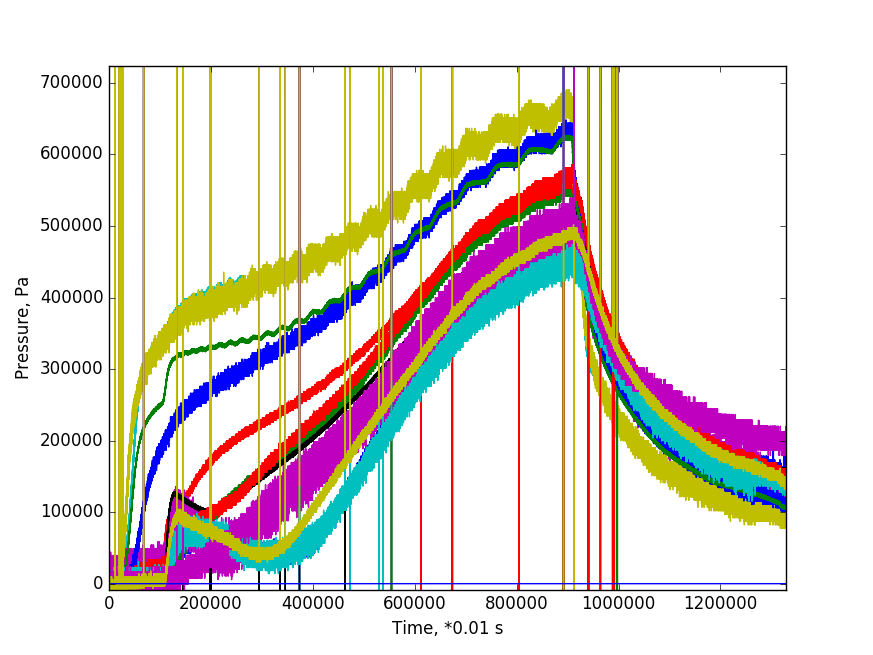
\epsfig{file=figs/picts/6, width=.5\textwidth}
\end{center}
\caption{Кривые давления в датчиках порового давления}\label{device4:pict}
\end{figure}

\section{Постановка задачи}
\subsection{Граничные условия для задачи упругости}

Схематеческий вид образца с прикладываемыми нагрузками представлен на рисунке~\ref{device5:pict}. На верхнюю поверхность образца прикладывалась вертикальная нагрузка перпендикулярно поверхности, поэтому вектор приложенной силы равен нормальной компоненте силы: $\vc{f}=\vc{f_n}=\sigma_n*\vc{n}$, где $\sigma_n=P_\text{top}$. Следовательно, на верхнюю поверхность ставится граничное условие Неймана на нормальное напряжение, равное вертикальной нагрузке: $\sigma_n = P_\text{top} = 20~atm$.

\begin{figure}[hb]
\begin{center}
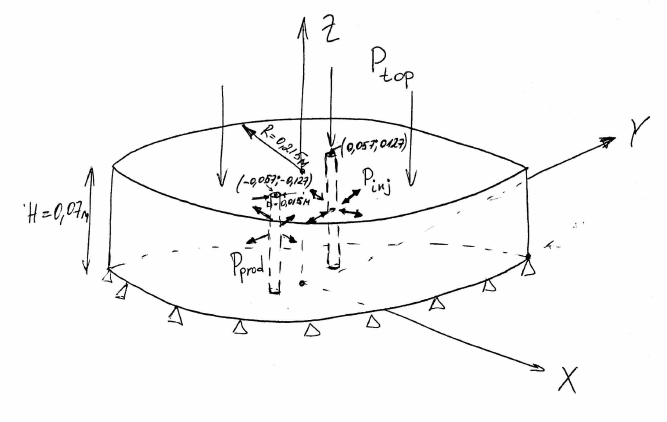
\epsfig{file=figs/picts/7, width=.4\textwidth}
\end{center}
\caption{Схематический вид образца с приклываемыми нагрузками}\label{device5:pict}
\end{figure}

Нижняя крышка установки зафиксирована жестко по вертикали, следовательно нижняя поверхность образца не может перемещаться вдоль оси $\mathcal{OZ}$ под действием вертикальной нагрузки. Таким образом, на низ образца ставится граничное условие Дирихле на перемещение (нулевое) по оси  $\mathcal{OZ}$: $u_z = 0$.

Чтобы исключить поворот образца вокруг своей оси и сдвига образца в плоскости $\mathcal{OXY}$. Для исключения таких перемещений можно поставить граничное условие Дирихле на всю боковую поверхноть образца в виде нулевого касательного перемещения в плоскости XY: $\vc{u}*\vc{e_\tau}=0$, где  $\vc{u}=(u_x, u_y, u_z)$, $\vc{e_\tau}=(-n_y, n_x, 0)$. То есть, граничное условие может быть переписано в виде: $-n_y*u_x + n_x*u_y=0$

Так же к граничным условиям для задачи упругости необходимо добавить условия на вспомогательные скважины, которые следуют из того факта, что в нагнетательную скважину закачивается жидкость под давлением, а добывающая связана с атмосферой. Таким образом, на скважины необходимо поставить условие Неймана на нормальные напряжение. На нагнетательную: $\sigma_n = P_\text{inj}=14.5~atm$; на добывающую: $\sigma_n =P_\text{prod}=1~atm$.

\subsection{Граничные условия для задачи фильтрации}

На верхнюю, нижнюю, боковую поверхности образца ставится условие непротикания. Это условие означает нулевой поток через данные поверхности, который, в свою очередь линейно зависит от градиента давления. То есть, граничное условие представляет собой условие Неймана на давление: $ \partial P/\partial\vc{n} = 0$

На вспомогательные скважины сначала задаются постоянные давления: в нагнетательную скважину закачивается раствор гипса под давлением 14.5 атм, а добывающая скважина связана с атмосферой. После установления стационарного режима закачка раствора в нагнетательную скважину прекращается, а добывающая скважина так же связана с атмосферой. Таким образом, на всю поверхность нагнетательной скважины с координатами  $(0.057, 0.127 )$ ставится граничное условие Дирихле: $P_\text{inj}=14.5~atm$ до достиженя стационарного режима. Далее, когда подача раствора прекращается, на нее ставится уже условие Неймана  $ \partial P/\partial\vc{n} = 0$ до конца эксперимента. На добывающую скважину с координатами  $(-0.057, -0.127 )$ ставится граничное условие Дирихле в течение всего эксперимента: $P_\text{prod}=1~atm$.

\section{Численный эксперимент}

